\startcontents[localtoc]
\printcontents[localtoc]{}{0}{\section*{Contents}\setcounter{tocdepth}{2}}



\phantomsection
\addcontentsline{toc}{section}{Overview}
\subsection*{Overview}



The example shows how nonscalar quantities can be used in variations and
plotting.



\phantomsection
\addcontentsline{toc}{section}{Inputs}
\subsection*{Inputs}



All input quantities are vectors. First value is x commponent, second value is
y component. Gravity acceleration is approx. [0, -9.81].
Starting velocity (m/s):

\begin{lstlisting}
DI.v.v = [0 0];
DI.v.u = [0 0];
\end{lstlisting}


Evaluation will be conducted at times (s):

\begin{lstlisting}
DI.t.v = [0 1 2 3];
DI.t.u = [0.1 0.2 0.3 0.4 0.5].*0.0001;
\end{lstlisting}


Varied input quantities:
Starting velocity is for 3 cases:
 1, still object,
 2, object thrown upward,
 3, object thrown forward,
 4, object thrown backward:

\begin{lstlisting}
DIvar.v.v = [0 0; 0 10; 10 0; -10 0];
\end{lstlisting}


Variation for velocity uncertainties: none, small, large:

\begin{lstlisting}
DIvar.v.u = [0 0; 0.2 0.2; 10 100];
\end{lstlisting}


Variation: Results calculated for short range of times and distant times:

\begin{lstlisting}
DIvar.t.v = [0 1 2 3; 4 5 6 7];
\end{lstlisting}


Some optional settings:

\begin{lstlisting}
CS.verbose = 1;
CS.mcm.repeats = 10;
CS.var.dir = 'qwtbvar_example_2_calculation_data';
CS.var.cleanfiles = 1;
CS.var.method = 'singlecore';
CS.var.procno = 1;
\end{lstlisting}


\phantomsection
\addcontentsline{toc}{section}{Calculation}
\subsection*{Calculation}



Run whole calculation. Input quantities in DI will be varied according DIvar:

\begin{lstlisting}
[jobfn] = qwtbvar('calc', 'qwtbvar_example_2_process', DI, DIvar, CS);
\end{lstlisting}
\begin{lstlisting}[language={},xleftmargin=5pt,frame=none]
### QWTBVAR: Number of variation calculations is: 24
### QWTBVAR: All calculations finished. The calculations took 0.00832 s (0.000139 m, 2.31e-06 h)

\end{lstlisting}


\phantomsection
\addcontentsline{toc}{section}{Results}
\subsection*{Results}



Get results as multidimensional arrays, where every dimension represents one
varied quantity. The result will be for selected settings of consts.

\begin{lstlisting}
qwtbvar('plot2D', jobfn, 'v.v', 'range.v');
consts.v.v = [0   0];
consts.v.u = [0   0];
qwtbvar('result', jobfn, consts);
qwtbvar('plot2D', jobfn, 'v.v', 'range.v', consts);
qwtbvar('plot3D', jobfn, 'v.v', 'v.u', 'range.v', consts);



% % consts.v.v = [1 2];
% consts.v.u = [0.1 0.2];
% [ndres, ndresc, ndaxes] = qwtbvar('result', jobfn, consts);
% % ndres is a structure with results as matrices. Although, because results are not scalars,
% % it contains cells.
% % ndresc is a cell with structures of results.
% % ndaxes is description of which quantity was varied in which dimension.
\end{lstlisting}
\begin{center}
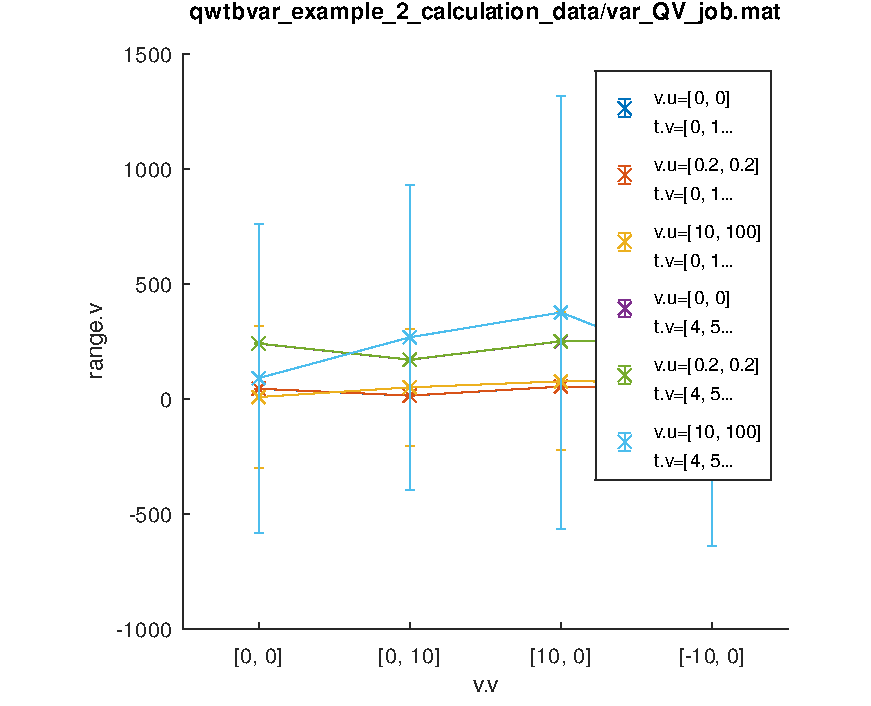
\includegraphics[width=0.7\textwidth]{qwtb_examples_published/qwtbvar_example_2-1.pdf}
\end{center}
\begin{center}
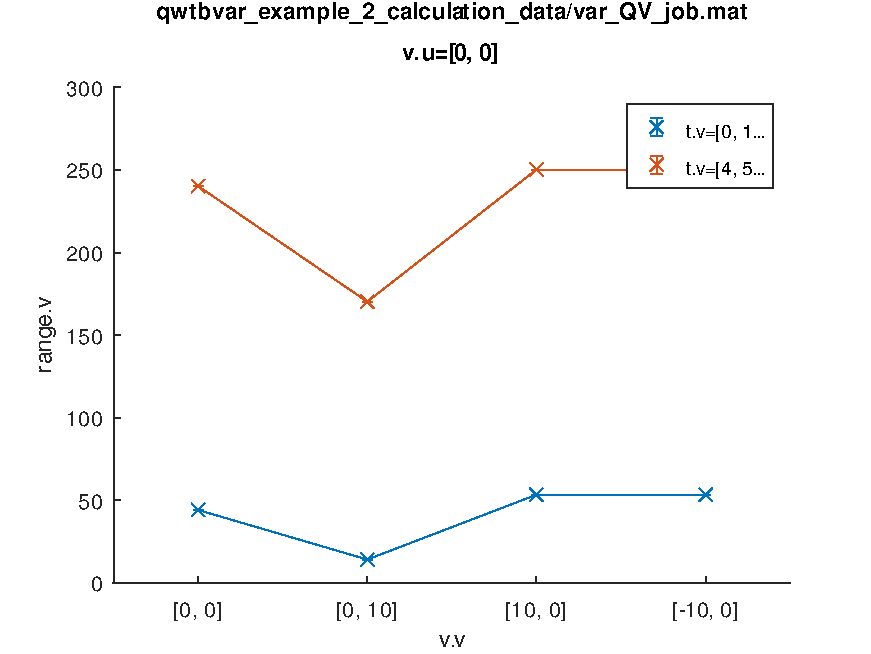
\includegraphics[width=0.7\textwidth]{qwtb_examples_published/qwtbvar_example_2-2.pdf}
\end{center}
\begin{center}
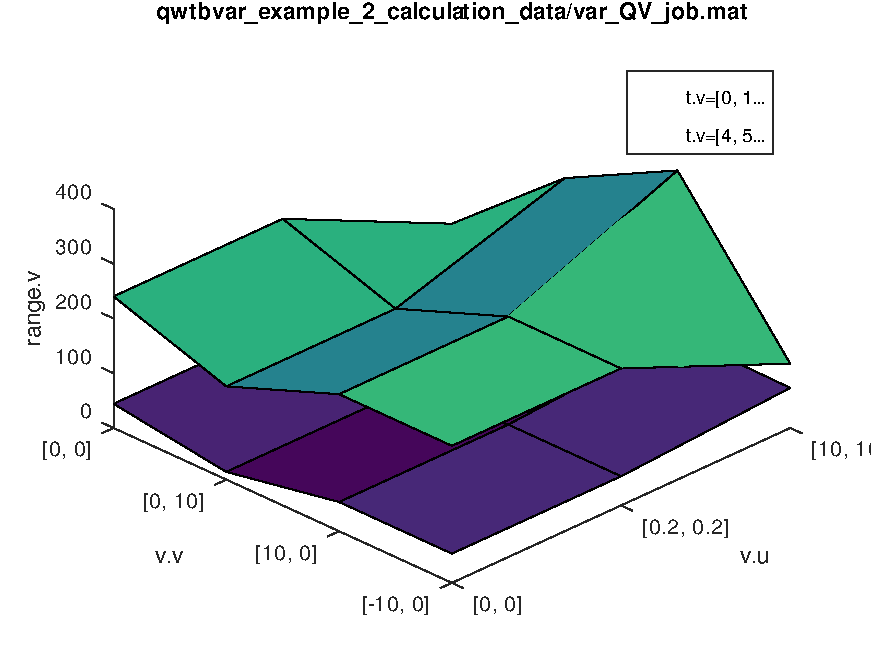
\includegraphics[width=0.7\textwidth]{qwtb_examples_published/qwtbvar_example_2-3.pdf}
\end{center}


\stopcontents[localtoc]
